
\part{Stochastic Jump Processes and Applications} %%% part I

\chapter{Stochastic Jump Processes}\label{chap1}%Chap 1


\setcounter{section}{-1}
\section{Introduction}%section 0

Stochastic\pageoriginale jump processes  are processes  with piecewise
constant paths. The Poisson process, the processes  arising in
Inventory problems  (stocks of  items in a store with random  ordering
and replacement) and queuing  systems  (arrivals at a queue with each 
customer having  random demand for service) are examples of
stochastic jump processes. Our aim here is to develop a theory
suitable for studying optimal control of  such processes. 

In Section \ref{chap1:sec1}, martingale theory and stochastic calculus  for jump
processes are  developed. Gnedenko-Kovalenko \cite{key16} introduced
piecewise-linear process. As  an example of such a  process, consider
virtual waiting time process $(VWT)$  for queueing systems, where $VWT
(t)$   is the  time customer arriving  at time  $t$ would have to wait
for service, see Fig.~(\ref{chap1:fig1}). 

Later Davis \cite{key7} and  Vermes  \cite{key25} introduced the
concept of piecewise 
deterministic processes which follow smooth curves (not necessarily
straight lines) between jumps. In Section \ref{chap1:sec2}, we will study some
applications to piecewise-deterministic processes. The idea there is
to  derive Markov properties, Dynkin's formula, infinitesimal
generators etc., using the  calculus developed in Section \ref{chap1:sec1}. 

\begin{figure}[H]
\centering
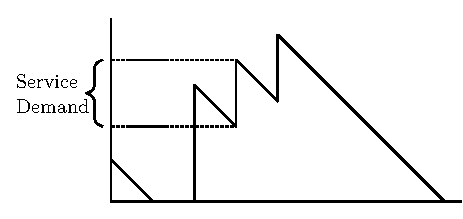
\includegraphics{vol75-figures/fig1.eps}
\caption{Arrival time of customers}\label{chap1:fig1}
\end{figure} \pageoriginale

\setcounter{section}{0}
\section{Martingale Theory for Jump Processes}\label{chap1:sec1}%%% 1

Let $(X, S)$ be a Borel space.

\begin{defn}%%% 1
  A jump process is defined by sequences  $ T_1, T_2, T_3$, $\ldots$,
  $Z_1, Z_2, Z_3,  \ldots $ of random variables,  $ T_i \in 
  \mathbb{R}_+ $ and   $ T_{i+1} > T_i$ a.s. and  $ Z_i \in 
  (X,S)$. Set  
  $$
  T_{\infty} = \lim_{ k \rightarrow \infty}  T_k.
  $$
\end{defn}

Let $z_0, z_\infty  $  be  fixed elements of $X$. Define the path $
(x_t)_{t \geq 0}$ by 
$$
x_t =  
\begin{cases}
  z_0  & \text{if} \quad  t < T_1 \\
  Z_i  & \text{if} \quad t \in  [T_i, T_{i+1} [ \\
  z_\infty  & \text{if} \quad t \ge T_\infty. \\
\end{cases}
$$

Then the probability structure on the process is determined by either
joint distribution for $ (T_i, Z_i, i = 1,2, \ldots) $ or
specifying  
\begin{enumerate}[(i)]
\item  distribution\pageoriginale of $(Z_1, T_1) $ 
\item for each $ k = 1,2, \ldots, $ conditional distribution of  $
  (S_k, Z_k \mid T_{k-i}, i = 1, 2, \ldots )$, where  $ S_k =
  T_k-T_{k-i} $  is  then $ k^{\text{ th }} $  inter-arrival time. 
\end{enumerate}

We will start  studying  the  process  $(x_t) $ having a single jump,
i.e., 
$$
x_t
\begin{cases} 
  z_0 & \text{if} \quad  t < T (\omega)\\
  Z_{(\omega)}  & \text{if} \quad  t \ge  T (\omega).
\end{cases}
$$
If  $T=\infty $, let $Z= z_\infty $, a fixed point of $X$.

\begin{figure}[H]
\centering
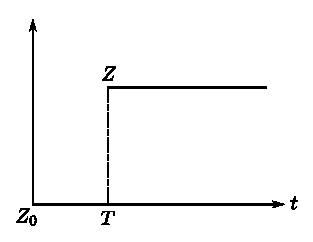
\includegraphics{vol75-figures/fig2.eps}
\caption{}\label{chap1:fig1.2}
\end{figure}

Define  the probability space  $(\Omega, F, P ) $ as  the canonical
space for $T$, $Z$, 
$$
\displaylines{\text{i.e., }\hfill
(( \mathbb{R}_+ \times X) U \{ ( \infty, z_\infty)\}, B ( \mathbb{R}_+
)~   *  S, \{ ( \infty, z_\infty)\}, \mu ) }
$$
where  $ \mu $ is a probability measure on 
$$
(( \mathbb{R}_+ \times X) U \{ ( \infty, z_\infty)\}, B ( \mathbb{R}_+
)~*S,\{(\infty, z_\infty)\}). 
$$
The\pageoriginale random function  $(x_t)$  generates the  increasing
family of  $\sigma - $ fields  $(F_t^0)$, i.e., 
$$
F_t^0 = \sigma \{ x_S, s \leq t \}.
$$
We suppose 
$$
\mu (( [ 0, \infty ] \times \{z_0 \} ) U \{ 0 \}  \times X) = 0. 
$$
This assumption guarantees that the process  $x_t$ does jump at its
jump time $ T $, i.e., 
$$
P( T > 0 \text{ and  } ~  Z \neq z_0 ) = 1.
$$

Recall that an $\mathbb{R}_+ $ - valued random variable $ \tau $ is a
stopping time of a filtration $ F_t, $ if  $ (\tau \leq t  \in) 
F_t, \forall t $. Let  
$$
F_t = \text{ Completion of } F_t^0  ~ \text{ with all } F_\infty^0  -
\text{ null sets }. 
$$

\begin{prop}%Prop 1.1
 $T$  is not an $F_t^0 $ stopping time, but $T$ is an $F_t $ stopping
  time.   
\end{prop}

\begin{proof}
Let $ A = \{ Z = z_0 \}$  and  $K$ be any set in $X$. Then
$$
\displaylines{
x^{-1}_{S} (K) = \hfill \cr
\begin{cases}
([s, \infty ] \times X) U ([ o,s ]  \times \{ z_0 \} ) &~\text{ if }~
    z_0 \in  K ~\text{ and } ~Z( E - A ) \cap K = \phi \\ 
((s, \infty ] \times X) U ([ o,s ]  \times K ) &~\text{ if }~ z_0
  \in  K ~\text{ and } ~Z( E - A ) \cap K  \neq  \phi. \\ 
[ o,s ] \times K    &~\text{ if } z_0 \not\in  ~  K.\\
\end{cases} }
$$
where  $E  = \mathbb{R}_+  \times X - A $.

Clearly $[ 0, t ] \times X $ cannot be in the  $ \sigma $- algebra
generated  by sets of the  above form. So $T$ is not  an $ F_t^0 $
stopping time. Let $ B = X - \{z_0 \} $. By assumption, $ P (A) = 0
$; so $ A \in  F_t $.  
$$
x^{-1}_{t} (B) = [ 0,t] \times X-A \in  F_t^0.
$$
So\pageoriginale
$$
[ 0, t ] \times X \in  F_t.
$$
But  $ \{ T \leq t \}  = [ 0, t ] \times X $. Hence  $ T $ is an $
F_t $  stopping time.
\end{proof}

It can be seen that
$$
 F_t = B[ o, t ] ~ * S U (]t, \infty]\times X )  U  ~\text{ null sets
      of } F_\infty^\circ. 
$$

The stopped $ \sigma $- field  $ F_T $ is  given by 
$$
F_T = \{ G \in  F_\infty : G \cap (T \leq t ) \in  F_t,
\forall t  \}. 
$$ 
Clearly
$$
F_T = F_\infty.
$$


\setcounter{definition}{1}
\begin{definition}%Def 1.2
  A process  $ ( M_t ) $ is an $F_t $ -martingale if $ E \mid M_t \mid
  < \infty $  and for  $ s \leq t $ 
  $$
  E [ M_t \mid F_s ] = M_s ~  \text{a.s.}
  $$
  
  $( M_t ) $ is a local $F_t $- martingale if there exists a sequence
  of stopping times $ S_n \uparrow \infty$ a.s. such that $ M^n_t : =
  M_{t \Lambda S_n} $ is a  uniformly integrable  martingale  for
  each $n$; here  $ t \Lambda S_n : = Min ( t, S_n ) $. 
\end{definition}

\begin{prop}%Prop 1.2
  If  $ M_t $ is a  local martingale and   $S$ is a stopping time  such
  that   $S \geq T$   a.s.,  then  $ M_S = M_T$   a.s.
\end{prop}

\begin{proof}
  Let  $S_n$  be stopping times such that  $ S_n \uparrow \infty$ a.s.
  Then  $ M_{t \Lambda S_n } $ is $u. i$. martingale. Let $ M^n_t
  = M_{t \Lambda S_n }, \forall n  $.  Then by optional sampling
  theorem  
  $$
  \displaylines{\hfill
    E [ M^n_S  F_{ T \Lambda S_n } ] = M^n_T ;\hfill\cr
    \text{but}\hfill F_T = F_\infty.\hfill }
  $$  
  So\pageoriginale
  $$
  E [ M^n_S \mid  F_T ]  = M^n_S.
  $$
 Also
  $$
  \displaylines{\hfill
  \lim_{ n \rightarrow \infty} M^n_T = M_T\hfill \cr
  \text{and}\hfill 
  \lim_{ n \rightarrow \infty} M^n_S = M_S.\hfill }
  $$
 So
  $$
  M_S = M_T  ~ a.s.
  $$
\end{proof}

\begin{prop}\label{chap1:prop1.3}%Prop 1.3
 Suppose $\tau $  is an $ F_t $-stopping time.  Then there
  exist $ t_0  \in  \mathbb{R}_+ $  such that $ \tauup  \Lambda
  T = t_0 ~  \Lambda T$ a.s. 
\end{prop}

\begin{proof}%Prf
  If $ \tau $  is  a stopping  time, then $(  \tau \Lambda T \leq t )
  \in  F_t,  \forall t$. But if  $ T \Lambda \tau $  is not
  constant a.s. on  $(\tau \leq T)$, then  
  $$
  (\tauup \Lambda T \leq t) \cap  (] t, \infty]  \times X )
    \underset{\neq}{\subset} ]t, \infty[ \times X \text{ for some }~ t
        \in  \mathbb{R}_+. 
        $$
        But  $[t, \infty ]  \times X $  is an atom of  $ F_t $. This
        contradicts the fact that  $ \tau $ is a  stopping time. So 
        $$
        \tau  \Lambda T = t_0  \Lambda T a.s.
        $$

The general definition of a stopped  $ \sigma $-field is that if $U$
is a stopping time. Then  
$$
F_U = \{ A  \in  F \mid A  \cap ( U  \leq t ) \in   F_t,
\forall t  \}. 
$$

But this is an implicit definition of the  $ \sigma $-field. 
\end{proof}

\begin{exercise}%Exerc 1.1
  Suppose  $\tau = t_0  \Lambda T $. Show that 
  \begin{enumerate}[(i)]
  \item  $ F_{\tau} = F_{t_o}$
  \item  $ F_{\tau} = \sigma \{x_{\tau  \Lambda s}, S \ge 0  \}$.
  \end{enumerate}
\end{exercise}\pageoriginale

\begin{definition}%Def 1.3
  For  $ A \in  S $, define 
  $$
  \displaylines{\hfill 
    F^A ( t )  =  \mu ([ t, \infty ] \times A )  \hfill \cr
  \text{and}\hfill  
  F (t) = F^X ( t ) = P [ T > t ].\hfill} 
  $$

Note that  $ F ( 0 ) = 1  $ and  $ F (. )$ is  monotone decreasing
and  right continuous. Define  
$$
c= 
\begin{cases}
\inf  ~ \{ t : F (t) =  0  \} \\
+ \infty ~ \text{ if }  ~ \{ t : F(t)  = 0 \}  = \phi .
\end{cases} 
$$
\end{definition}

\begin{prop}\label{chap1:prop1.4}%Prop 1.4
  Suppose $ (M_t )_{t \geq  0 } $  is an $ F_t $  local martingale.  Then
  \begin{enumerate}[(a)]
  \item  if $c = \infty $  or $ c < \infty $  and $ F(c- ) =  0 $,
    then $ M_t $  is a martingale on $ [ 0,c [ $. 

    \item  if $c<\infty, F (c-) > 0 $,  then $ (M_t )$  is a
      uniformly integrable martingale. Here $ F ( c- ) = \lim\limits_{
        t \uparrow c} F (t) $.  
  \end{enumerate}
\end{prop}

\begin{proof}%Prf
  \begin{enumerate}[(a)]
  \item  If  $ \tau_k \ge T a.s $. for some  $k$, then 
    $$
    M_{t  \Lambda \tau_k} = M_{t \Lambda \tau _k \Lambda T} = M_{t \Lambda T} = M_t.
    $$

    So $M_t$ is a  $u.i$. martingale. Hence suppose $P[ \tau_k   <
      T] > 0 $ for all $ k (*)$; then by Proposition \ref{chap1:prop1.3}, 
    $$
    \tau_k \Lambda T = t_k  \Lambda T ~  \text{ for some fixed }  t_k
    $$
    and\pageoriginale  $t_K <c $ because of  $(*)$. Also $t_k
    \uparrow c $ since  $\tau_k \uparrow \infty $. 

    So
    $$
    M_{t  \Lambda \tau_k} = M_{ t \Lambda \tau_k \Lambda T} =  M_{t
      \Lambda T \Lambda t_k}  =  M_{ t \Lambda t_k}. 
    $$ 

    Hence $M_{t \Lambda t_k }$ is a u.i. martingale. So $ (M_t)_{t
      < c } $  is a  martingale.  

  \item $ c  < \infty,  F ( c_- )  > 0 $.
  $$
  F(c_-) = P( T = c )
  $$

  $P (T = c) >  0 $; so it must be the case that  $ t_k = c $ for
  some $k$. Otherwise  $ P (\tauup_k < c ) \ge ~  F (c- ) > 0 $; so
  ``$\tauup _k \uparrow \infty \; a.s.$'' fails. For this  $k$,  
  $$
  M_{t \Lambda t_k } =  M_t
  $$
  \end{enumerate}
So $(M_t)$ is  a $ u.i $. martingale. 

Our main objective is to show  that  all local martingales can be
represented  in the form of  ``stochastic  integrals''. So we
introduce some ``elementary martingales''  associated with the
process $(x_t) $. For $ A \in  S $ and  $ t  \in 
\mathbb{R}_+ $, define 
\begin{align*}
  p ( t,A ) ~ &= \tilde{I}_{(t \ge T)} I_{( Z \in  A )} \\
  \tilde{p} ( t,A ) ~ &= -\int\limits_{ ]o,T \Lambda  ~t[} \frac{1}{F
    (s_- )} dF^A (s).\\ 
\end{align*}
\end{proof}

\begin{prop}\label{chap1:prop1.5}%%% 1.5
  Let $ q (t,A)    = p(t,A)-\tilde{p} (t,A) $. Then $ (q (t,A))
  _{t \ge 0 } $  is an $ F_t $  - martingale,  i.e., $ \tilde{p (t,A)}
  $  the ``compensator'' of the point process $ p (t,A) $. 
\end{prop}

\begin{proof}
  (Direct calculation).\pageoriginale Take $ t > s $, then   
  \begin{align*}
    E & [ p(t,A) - p (s,A)  \mid F_s ] = I_{(s < T)} \frac{ F^A (s) -
      F^A (t)}{F(s)}.\\ 
    E & [ \tilde{p}(t,A) - \tilde{p} (s,A)  \mid F_s ] = I_{s < T }\\ 
    & \qquad \quad\left\{\frac{F (t)}{F (s)} \int \limits_{[s.t ]}
    \frac{dF^A (u)}{F (u-)}  - \frac{1}{F (s)} \int \limits_{[s.t ]}
    ~ \int \limits_{[s.r]} \frac{ dF^A (u)}{F (u-)} dF (r) \right\} 
\end{align*}
and
\begin{align*}
  \int \limits_{[ s,t ]} ~ \int \limits_{[ s,r ]} \frac{ dF^A (u)}{F
    (u-)}dF(r) ~ &= \int\limits_{[s, t]}\frac{1}{F (u-)} \int
  \limits_{[ u,t ]} dF (r) dF^A (u)\\ 
  &= \int \limits_{[ s.t ]} ~  \frac{1}{F (u-)} (F (t) - F
  (u-)) dF^A (u) \\ 
  &= F (t) \int \limits_{[ s.t ]} ~ \frac{ dF^A (u)}{F (u-)} ~ +  F^A
  (t) - F^A (s). 
\end{align*}
So
$$
E [ q (t, A) - q (s, A) \mid  F_s ]  = 0 
$$
\end{proof}


\medskip
\noindent{\textbf{Another  expression for  {\boldmath$\tilde{p}(t,
      A)$}:}}
 We have $ F^A (.) <<  F
(.)$  (i.e. $F^A\, (.)$ is absolutely continuous  w.r.t. $F (.)$). So
there exists a function $\lambda (s,A)$ such that  
$$
F^A (0) - F^A (t) = - \int \limits_{] o.t ]} ~ \lambda (s,A ) d F (s). 
$$

In fact
$$
\lambda (s,A) = P (Z \in  A  \mid T  = s ).
$$

Suppose $X$ is such that a regular version of this conditional
probability exists (which is the case, since $X$ is Borel
space). Then $ \dfrac{- dF^A (s)}{F (s-)} ~ = \lambda (s,A) d \Lambda
(s) $ 
where $ d \Lambda (s)  \dfrac{- dF (s)}{F (s-)} $. 

Then  
$$
\tilde{p} (t,A) =  \int \limits_{] o, T ~ \Lambda ~ T ]}  \lambda
    (s,A) d \Lambda (s). 
$$

\medskip
\noindent{\textbf{Stochastic  Integrals}}\pageoriginale

Let  $I$ denote the set of measurable functions $ g : \Omega
\rightarrow \mathbb{R} $ such that  $ g ( \infty, z_\infty ) = 0 $. 

\begin{enumerate}
\renewcommand{\theenumi}{\alph{enumi}}
\renewcommand{\labelenumi}{\bf (\theenumi)}
\item \textbf{Integrals  w.r.t. \boldmath{$p(t,A)$}:}
  Suppose $N_t$ is a counting process. Since its sample functions are
  monotone increasing and there is a one-to-one correspondence between
  monotone increasing functions and measures, and  since in this case,
  mass is concentrated at the jump points and they are only countable;
  the function $N_t$ defines a random measure on  $(\mathbb{R}, B (
  \mathbb{R})) $ say, $ \pi = \sum \limits_{i} \delta _{T_{i}} $ where
  $ \delta_X $ is the  Dirac measure at  $x$. Similarly, the one jump
  process can be identified with the random measure  $ \delta_{ (T,x_T
    )}$ on $ R_+  \times X $. So we can define Stieltjes integrals of
  the form $ \int g (t,x )   p (dt,dx) $ for suitable integrands $ g
  \in  I $ as  
  $$
  \int \limits_{\Omega} g (t,x)\, p (dt,dx) = g (T, x_T).  
  $$ 
  We say  $g \in   L_1 (p)$ if 
  $$
  E \int\limits_{\Omega} |g (t,x) \mid  p(dt,dx)  < \infty  
  $$
  and denote
  $$
  \mid\mid g \mid\mid_{L_1 (p)} = E \int \limits_{\Omega} \mid g 
  (t,x) \mid p (dt,dx)  
  $$

  Clearly $g \in  L_1 (p) $  if and only if 
  $$
  \int \limits_{ \mathbb{R}_+ \times X} \mid g (t,x)  d \mu  < \infty  
  $$

\item \textbf{Integrals  w.r.t. {\boldmath$\tilde{p} ( t,A
    )$}:}\pageoriginale 

  Recall  $ \tilde{p} (t,A)  =  \int \limits _{] o, T  ~ \Lambda ~ t]}
  \lambda (s,A) d \Lambda (s) $. 

  So we define
  $$
  \displaylines{\hfill
  \int \limits_{\Omega} g (t,x) \tilde{p} (dt,dx ) = \int \limits_{[
  o, T ] }  \int \limits_{X} g (t,x) \lambda (t,dx) d \lambda (t)
    \hfill \cr
    \text{and say }\hfill 
    g \in  L_1 ( \tilde{p} ) ~ \text{ if } \int\limits_\Omega ~|g (t,x) \mid
    \tilde{p} (dt,dx )  < \infty  \hfill \cr
    \text{and}\hfill  
    \mid\mid g \mid\mid_{L_{1} ( \tilde{p})} =  \int \limits_{\Omega}
    \mid  g (t,x) \mid \tilde{p} (dt,dx ).\hfill }
  $$
\end{enumerate}


\begin{prop}%Prop 1.6
  $$
  \mid\mid g \mid\mid_{L_{1} ( p)} = \mid\mid g \mid\mid_{L_{1} (
    \tilde{p})}
$$
and so 
$$
L_{1} (p) = L_1 (\tilde{p}).
$$
\end{prop}

\begin{proof}
  \begin{align*}
    \mid\mid g \mid\mid_{L_{1} ( \tilde{p})} &= -  \int
    \limits_{\mathbb{R}_+} \int \limits_{[o, T ] } \frac{1}{F (s_-)}
        \mid g (s,x)  \mid d \mu (s,x) d F (T) \\ 
        &= \int \limits_{\Omega} \frac{1}{F (s_-)} \mid g (s,x)\mid( -\int
        \limits_{[ s, \infty ]} d F(t)) d \mu (s,x) \\ 
        &= \int \limits_{\Omega} \mid g (s, x) \mid d\mu (s,x) \\
        &= \mid\mid g \mid\mid _{L_{1} (p)}.
  \end{align*}

Define
\begin{align*}
  L^{\loc}_{1} (p) &=  \{ g \in  I \mid g (s,x) I_{s \leq t }
  \in  L_{1} (p), \forall t < c \} \\ 
  L^{\loc}_{1} (\tilde{p} ) &= \{ g \in  I \mid g (s,x) I_{s
    \leq t } \in  L_{1} (p), \forall t < c \}. \text{ Clearly }
  \\ 
 L^{\loc}_{1} (p) &= L^{\loc}_{1} (\tilde{p} ).
\end{align*}

Following\pageoriginale is the main result of this section, which
gives an integral representation for $F_t$ local martingales. 
\end{proof}

\begin{prop}\label{chap1:prop1.7}%Prop 1.7
  All $ F_t$-local martingales are of the form 
  \begin{align*}
    M_t &= \int \limits_{\Omega} (g (s,x) I_{(s \leq t)} dq(s,x) \\
    &= \int \limits_{\Omega} (g (s,x) I_{s \leq t} dp(s,x) -\int
    \limits_{\Omega} (g (s,x) I_{(s \leq t)} \tilde{dp}(s,x). 
  \end{align*}
for some $g\in  L^{\loc}_{1} (p) $.
\end{prop}

We need the following result.

\begin{lemma}% lem 1.1
  Suppose  $(M_t)_{t > 0} $ is $ u.i. F_t$ martingale with $ M_0 = 0
  $. Then there exists a function  $ h: \Omega \rightarrow \mathbb{R} $
  such that 
  \begin{equation*}
    E \mid h (T, Z ) \mid < \infty \tag{1}\label{chap1:sec1:eq1}
  \end{equation*}
  and
  \begin{equation*}
    M_t = I_{( t \ge T )} h (T,Z) -I_{(t < T)} \frac{l}{F (t)} \int
    \limits_{] 0, t] \times X } h (s,z) \mu (ds,dz)
        \tag{2}\label{chap1:sec1:eq2}  
  \end{equation*}
\end{lemma}

\begin{proof}
  If $ (M_t)$ is a $u.i$. martingale, then $ M_t = E [ \xi \mid ~ F_t
  ] $ for some $ F_\infty $-measurable  r.v. $\xi $ and from the
  definition of $ F_\infty $, we have 
  $$
  \xi = h ( T, Z )~ a.s.
  $$
  for some measurable  $ h : \Omega \rightarrow  \mathbb{R}
  $. Expression (\ref{chap1:sec1:eq1}) is satisfied
  since\pageoriginale $M_t$ is u.i.,   and $M_o = 0$ implies   
  \begin{equation*}
    \int \limits_\Omega h. d \mu = 0. \tag{3}\label{chap1:sec1:eq3}
  \end{equation*}

Now
\begin{align*}
  M_t & = E[h(T, Z)|F_t] \\
  & = I_{(t \geq T)} h(T, Z) + I_{(t < T)} \frac{1}{F(t)}
  \int\limits_{] t, \infty ] \times X} h(s,x) \mu (ds,
      dx). \tag{4}\label{chap1:sec1:eq4}   
\end{align*}

From (\ref{chap1:sec1:eq3}) and (\ref{chap1:sec1:eq4}), we have
(\ref{chap1:sec1:eq2}). 
\end{proof}

For $g \in  L^{\loc}_I (p)$, the stochastic integral 
$$
M^g_t = \int \limits_{] 0,t ] \times X} {g(s,x) q(ds,dx)}
$$
is defined by
$$
M^g_t = \int \limits_{\mathbb{R}^+ \times X} I_{(s \leq t)}
    g(s,x) p(ds,dx)- \int \limits_{\mathbb{R}^+ \times X} I_{(s \leq
      t) g(s,x)} \tilde{p}(ds, dx). 
$$

Then the question is whether $M_t$ given by (\ref{chap1:sec1:eq2}) is
equal to $M^g_t$ for some $g$. As a motivation to the answer consider
the following example.	 

\begin{example}\label{chap1:exam1.1}%exe 1.1
  Let $(X, S) = (\mathbb{R}, B(\mathbb{R}))$ and 
  $$
  \mu (ds, dx) = \psi(s,x) ~ds ~dx.
  $$
\end{example}

Then 
\begin{multline*}
  M^g_t  = I_{(t \ge T)} \left\{ g(T,Z) - \int \limits^T_0 \int
  \limits_{\mathbb{R}} \frac{1}{F(s)} g(s,x) \psi (s,x)dx ds \right\} \\ 
  -  I_{(t \ge T)} \left\{ \int \limits^t_0 \int\limits_{\mathbb{R}}
  \frac{1}{F(s)} g(s,x) \psi (s,x)dx ds \right\} \tag{5}\label{chap1:sec1:eq5} 
\end{multline*}

If\pageoriginale $M^g_y$ given by (\ref{chap1:sec1:eq5}) is equal to
$M_t$ given by (\ref{chap1:sec1:eq2}), then the coefficients of $I_{(t
  \ge T)}$ and $I_{(t < T)}$ must agree. Comparing the coefficients of
$I_{(t > T)}$, we require    
$$
h(t,z) = g(t,z) - \int \limits^t_0 \int \limits_{\mathbb{R}}
\frac{1}{F(s)} g(s,x) \psi (s,x)dx ds.  
$$
Let 
$$
\eta(t) = h (t,z) - g(t,z).
$$
Define
$$
\gamma(t) =  \int \limits_{\mathbb{R}} \psi h dx
$$
and  
$$ 
f(t) =  \int \limits_{\mathbb{R}} \psi dx.
$$
Then
\begin{align*}
  \eta(t) & = \int \limits^T_0 \frac{1}{F(s)} \left(\int \limits_{\mathbb{R}} h
  (s,z) + \eta (s)\right) \psi (s,x)dx) ds \\ 
  & = \int \limits^t_0 \frac{1}{F(s)} \gamma(s)ds + \int \limits^t_0
  \frac{1}{F(s)} \eta(s)f(s)ds; 
\end{align*}
that is 
\begin{align*}
  \frac{d}{dt} \eta(t)&  = \frac{f(t)}{F(t)} n(t) + \frac{1}{F(t)}
  \gamma (t) \\ 
  \eta(o) & = 0
\end{align*}
which has a unique solution
$$
\eta(t) = \int \limits^t_0 \phi (t,s) \frac{1}{F(s)} \gamma(s)ds,
$$
where
\begin{align*}
\phi(t,s) & = \exp \int \limits^t_s \frac{f(u)}{F(u)} du \\
& = \frac{F(s)}{F(t)}, ~\text{since}~ f(t) = - \frac{dF(t)}{dt}.
\end{align*}
So\pageoriginale 
$$
\eta(t) = \frac{1}{F(t)} \int \limits^t_0 \gamma(s)ds.
$$
Hence 
\begin{equation*}
  g(t,z) = h(t,z) + \frac{1}{F(t)} \int \limits^t_0  \int
  \limits_{\mathbb{R}} h(s,x) \psi (s,x)dx ds \tag{6}\label{chap1:sec1:eq6} 
\end{equation*}
Now it can be checked that with this choice of $g$ the coefficients of
$I_{(t < T)}$ in (\ref{chap1:sec1:eq2}) coincides with that of
(\ref{chap1:sec1:eq5}). So $M_t = M^g_t$. 

Now we can prove the general case given in Proposition
\ref{chap1:prop1.7}. 



\setcounter{proofofprop}{6}
\begin{proofofprop}%pro 1.7
  \begin{case}\label{chap1:case1}%cas 1
    $c < \infty, F(c_-) > 0$. Take a local martingale $M_t$ with $M_o =
    0$. Then $(M_t)$ is u.i. So $M_t = E[h (T,Z) | F_t]$ for some
    measurable $h$ such that $E|h| < \infty, E h = 0$. Then we claim
    that $M_t = M^g_t$ where 	 
    $$ 
    g(t,z) = h(t,z) + I_{(t < c)} \frac{1}{F(s)} \int \limits_{]\circ, t]
      \times x} h(s,z)\, \mu\, (ds, dz). 
        $$ 
  \end{case}
  
  But this can be seen algebraically following similar calculations as
  of the example \ref{chap1:exam1.1}. Now to show that $g \in  L^{\loc}_1
  (p)$. 
  \begin{align*}
    \int |g| d \mu & \le \int |h| d \mu - \int \limits_{]o, c [}
    \frac{1}{F(t)} \int \limits_{]o, t]\times X} |h|d \mu dF(t) \\ 
        & \le \int |h| d \mu - \frac{1}{F(c_-)} \int \limits_{]o, c [}
        \int \limits_{]o, t] \times X} |h|d \mu d F(t) \\ 
        & \le \int |h| d \mu + \frac{1}{F(c_-)} \int \limits_{]o, c
             [\times X} (F(t) - F(c_-)) |h| d \mu \\ 
        & \le \left(1 + \frac{1}{F(c_-)}\right) \int |h| d \mu <
             \infty. 
  \end{align*} 

  \begin{case}%cas 2
    $c = \infty$,\pageoriginale or $c < \infty$ and $F(c_-) = 0$. Then from
    proposition \ref{chap1:prop1.4}, $M_t$ is a martingale on $[ 0, c
    ]$, and so it 
        is u.i. on $[o,t]$ for $t < c$. Therefore 
        $$
        M_s = E[h (T,Z) | F_\infty]
        $$
        for some function $h$ satisfying 
   $$
        \int \limits_{] o, t ]x X}| g(s,x)| d \mu (s,x) < \infty
    ~\text{for all}~ t < c. 
    $$

    Define $g(s,x)$ as in (\ref{chap1:sec1:eq6}). Then calculations as in case
    \ref{chap1:case1}. Show that $M_s = M^g_s$ for $s \le t < c$. Now 
    \begin{align*}
      \int \limits_{[o,t ] \times X} |g|d\mu & \le \int \limits_{]o,t
      \times X} |h|d\mu -  \int \limits_{]o,t]} \frac{1}{F(s)}  \le
            \int \limits_{]o,s] \times X}|h|d\mu ~ dF(s)\\ 
                & \le \int \limits_{]o,t] \times X}|h|d\mu (1 - \int
                    \limits_{]o,t]} \frac{1}{F(s)} dF(s))\\  
                        & < \infty ~\text{for}~ t < c.
    \end{align*}
    Hence $g \in  L^{log}_1 (p)$.
  \end{case}
\end{proofofprop}

Conversely, suppose $g \in  L^{log}_1 (p)$. Then it can be
checked  that $M^g_t$ is a local martingale. 

\begin{remark}%Rem 1.1
  If $g \in  L^{log}_1 (p)$ then $M^g_t$ is a martingale. But
  the result does not say $M_t$ is a martingale if and only if $M =
  M^g$ for $g \in  L_{1} (p)$, it only characterizes {\em
    local} martingales. 
\end{remark}

\begin{remark}%rem 1.2
  All preceding results hold if $z_o$ is a random variable; then $\mu
  $ should be taken as conditional distribution of $(T,Z)$ given $z_o$ 
\end{remark}

\medskip
\noindent{\textbf{The multi-jump case:}}\pageoriginale
 The process $x_t$ has jump times $T_1, T_2, \ldots$ with
 corresponding states $Z_1, Z_2, \ldots$ Let ($Y,y$) denote the
 measurable space   
$$
(Y, y) = ((\mathbb{R}_+ \times X) U \{ ( \infty, z_\infty) \}, \sigma
\{ B (\mathbb{R}_+) * S, \{ (\infty, z_\infty) \} \}). 
$$
Define 
\begin{align*}
  \Omega & = \prod^{\infty}_{i = 1}Y_i , \Omega_K = \prod^{K}_{i = 1} Y_i \\
  F^o & = \sigma \left\{ \prod^{\infty}_{i = 1} y_i \right\} 
\end{align*}
where $(Y_i, y_i)$ denote a copy of $(Y, y)$. Let
$$
\displaylines{\hfill 
S_k (\omega) = T_k(\omega) - T_{k-1}(\omega)\hfill \cr
\text{and}\hfill 
w_k (\omega) = (S(\omega), Z_1(\omega), \ldots S_k (\omega), Z_k
(\omega)).\hfill }
$$
Then 
\begin{align*}
  T_k(\omega) &= \sum^k_{i = 1} S_i (\omega) \\
  T_\infty(\omega) & = \lim_{k \rightarrow \infty} T_k(\omega).
\end{align*}

As before, $(x_t(w))_{t \ge o}$ is defined by 
\begin{equation*}
  x_t(\omega)=
  \begin{cases}
    z_o & \text{if}~ t < T(\omega) \\ 
    Z_k & \text{if}~ t \in  [T_k(\omega),
      T_{k+1}(\omega)]\\ 
    z_\infty & \text{if}~ t \ge T_\infty(\omega) 
  \end{cases}
\end{equation*}

A probability measure $\mu$ on $(\Omega, F^o)$ is specified by a
family $\mu ^i : \Omega_{i-1} \times y \rightarrow [0,1]$ (with $\Omega_o
= \phi$) satisfying  
\begin{enumerate}[(i)]
\item $\mu ^i (.; \Gamma)$ is measurable for each fixed $\Gamma$
 
\item $\mu^i (w_{i-1}(\omega);.) $ is a probability measure on $(Y,
  y)$ for each fixed $\omega \in  \Omega$, 

\item $\mu^i (w_{i-1}(\omega);.(\{0\} \times X) \cup (\mathbb{R_+} \times
  \{ z_{i-1}(\omega)\})) = 0 $ for all $\omega$,\pageoriginale 

\item $\mu^i (w_{i-1}(\omega);.\{ (\infty, z_\infty)\}) = 1$ if
  $S_{i-1}(\omega) = \infty$. 
\end{enumerate}

Then for $\Gamma \in  y$ and $\eta \in  \Omega_{i-1}, \mu$
is defined by  
\begin{gather*}
  \mu [(T_1, Z_1) \in  \Gamma ] = \mu ^1(\Gamma) \\
  \mu [(S_i, Z_i) \in  \Gamma | w_{i-1} = \eta] = \mu^i (\eta :
  \Gamma) i = 2,3\cdots 
\end{gather*}

Notice that as in the single jump case, here (iii) ensure that two
``jump times'' $T_{i-1}, T$ do not occur at one and that the process
$x_t$ does effectively jump at its jump times (iv) ensures that $\mu
[Z_k = z_\infty | T_k = \infty] = 1$. 

As before, $F^{o}_{t} = \sigma \{ x_s, s \le t \}$ and 

$F_t =$ completion of $F^{o}_{t}$ with all $\mu$-null sets of $F^o$.

\begin{prop}%pro 1.8
  \begin{enumerate}[(i)]
  \item $F_\infty = F$, the completion of $F^o$

  \item $F_{T_n} = \prod \limits^n_{i-1} y_i \times \prod
    \limits^\infty_{i=n+1} y_i $. 
  \end{enumerate}
\end{prop}

The idea here is to reduce everything to one jump case. That is, the
process ``restarts'' at each $T_k$. We need the following result. 

\begin{prop}%pro 1.9
  $$
  F_{(T_{k-l} +t)} \Lambda T_k = F_{T_{k-l}} V \sigma \left\{ x_{(T_{k-l} +
    s)} \Lambda T_k, o \le s \le t)\right\}. 
  $$ 
\end{prop}

Proof of this is an application of the ``Galmarino test'' (Dellacherie
and Mayer \cite{key12}, theorem IV, pp. 100). 

Recall\pageoriginale that in one jump case $F_{t_o \Lambda T} = F_{t_o}$. Now we
conjecture that, if $U = (T_{k-1} + t_o) \Lambda T_k$, then  
$$ 
\displaylines{\hfill  
  F_U = \left(\prod^{k-1}_{i-1} y_i \right) * y^k_{t_o} * \left( 
  \prod^{\infty}_{i=k+1} Y_i \right),\hfill \cr  
  \text{where}\hfill
  y^k_{t_o}= S * B [o, t_o] \cup \left(x \times [t_o, \infty
  ]\right).\hfill } 
$$

As an example, see the following exercise.

\begin{exercise}%exe 1.2
  Consider a point process with $k = 2$, and take the probability
  space as $\mathbb{R}^2_+$. Then 
  $$ 
  x_t = \sum^2_{i=1} I_{(t \ge T_i)}.
  $$
\end{exercise}
Then 
\begin{enumerate}[(a)]
\item Show that 
  \begin{multline*}
    F_t= ~\text{Borel sets in}~ \{S_1 + S_2 \le t \}\\ 
  + (A \times \mathbb{R}_+) \bigcap B + [t, \infty] \times
  \mathbb{R}_+, A \in  B(\mathbb{R}) 
  \end{multline*}
  where
  $$
  B = \{ S_1 + S_2 \ge t \} \bigcap \{ S_2 \le t \}.
  $$

\item With $U = (T_1 +t_o) \Lambda T_2$, show that 
  \begin{multline*}
    F_U = B(\mathbb{R}_+ \times [o, t]) 
    + \{ (A \times \mathbb{R}_+) \bigcap ( \mathbb{R}_+ \times ] t_o,
      \infty ]) : A \in  B(\mathbb{R})\}. 
  \end{multline*}
\end{enumerate}

\medskip
\noindent{\textbf{Elementary Martingales, Compensator's}}
Define
$$
p(t,A) = \sum_{i} I_{(t \ge T_i)} I_{(z_i \in  A)}
$$
which counts the jump of $(x_t)$ ending in the set
$A$. Define
$$
\phi^A_1 (s) = - \int\limits_{[o,s ]}
  \frac{1}{F^1(u)} dF^{1A}(u)
$$\pageoriginale 
where
$$
  F^1 = \mu^1 ([t, \infty ] \times X)
$$
and
$$
  \phi^A_k (w_{k-1}; s) = - \int\limits_{[o,s]} \frac{1}{F^k(u_-)}
  dF^{kA}(u)
$$
where
$$
  F^{kA}(u) = \mu^k (w_{k-1}; [u, \infty] \times A).
$$
Now define
\begin{align*}
\tilde{p}(t,A) & = \phi^A_1(T_1) + \phi^A_2(w_1; S_2) + \cdots
\phi^A_j(w_{j-1}; t-T_{j-1}(\omega))\\
& \qquad \text{for }~ t \in  ]
  T_{j-1}, T_j ]. 
\end{align*}

\begin{exercise}%exe 1.3
  Consider a renewal process
  $$
  x_t = \sum_i I_{(t \ge T_i)} 
  $$
  and $S_i$'s are independent, $P(S_i > t) = F(t)$ is continuous. Then
  show that the compensator for $x_t$ is  
  $$
  \displaylines{\hfill  
  \tilde{p}(t) = - \ell n (F(S_1)F(S_2)\cdots F(S_{k-1}) F(t-T_{k-1})) 
  ~\text{for}~ t \in  [ T_{k-1}, T_k ],\hfill \cr 
  \text{and}\hfill  
      x_t - \tilde{p}(t)~\text{is a martingale.}\hfill}
      $$	
\end{exercise}

\setcounter{exam}{0}
\begin{exam}%exa 1
  If $F(t) = e^{- \alpha t}$, then $\tilde{p}(t) = \alpha t$.
\end{exam}

\begin{prop}%pro 1.10
  For\pageoriginale fixed $k$, and $A \in  S$,
  $$
  q(t \Lambda T_k,~~ A ) = p (t \Lambda T_k,~~ A)- \tilde{p} (t
  \Lambda T_k,~~ A), t \geq 0 
  $$ 
  is an $F_t$ -  martingale.
\end{prop}

\begin{proof}
  Calculation as in proposition \ref{chap1:prop1.5}.
\end{proof}

The  class of integrands $I$ consists of measurable function $g(t, x,
\omega)$ such that  
$$
g(t, x, \omega ) = 
\begin{cases}
  \quad g^1 (t,x ), & t \leq T_1 (\omega)\\
  g^k (w_{k-1}, t -T_{k-l}, x), &  t \in  ] T_{k-l} (\omega), T_k
    (\omega)],\\ 
      \qquad 0, & t \geq T_\infty (\omega )
\end{cases}
$$ 
for some function $g^k$ such that $g^1 (\infty, x ) = g^k (w_k;
\infty, x ) \equiv 0$. Such $g's$ are $F_1-$predictable
processes. Now we define $L_1 (p), L_1 (\tilde{p})$, etc. exactly as
in one jump case:  
\begin{align*}
  \int g\, dp &= \sum_i g (T_i, Z_i)\\
  L_i(p) & = \left\{ g \in  I : E \sum_i|g(T_i,Z_i)|< \infty
  \right\}\\ 
  \int g\, d \tilde{p}& = -\sum_k \int \limits_{ ]o, T_k -T_{k-l}]
    \times X} g(\omega_{k-l},s,x)\lambda (\omega_{k-l}, s,dx) 
      \frac{dF^k (s)}{F^k(s_-)} 
\end{align*}
where 
$$
\lambda(\omega_{k-l}, s,A) = \frac{dF^{kA}}{dF^k}(s)
$$
$g \in  \Gamma^{\loc}_1(p) $ if there exists a sequence of
stopping times $\sigma_k \uparrow T_\infty$ a.s. and $g I _{(t \leq
  \sigma_n } \in  L_1 (p), \forall n$. For $g \in 
L^{1oc }_1 (p)$ we define  
\begin{align*}
  M^g_t & = \int\limits_{[ o, t ] \times X} g(s,x)\, q\, (ds, dx)\\
      & =  \int\limits_{[ o, t ] \times X} g(s,x)\, p \,(ds, dx) -
          \int\limits_{[ o, t ] \times X} g(s,x)\, \tilde{p}\, (ds, dx). 
\end{align*}

\begin{prop}%pro 1.11
  If\pageoriginale  $g \in  L^{1oc}_{1}$ then there exists a
  sequence of stopping times $T_n < T_{\infty}$ such that $\tau_n
  \uparrow T_{\infty}$ and  $M^g_{t \Lambda T_n}$ is a 
  u.i. martingale for each $n$. 
\end{prop}

\begin{proof}
  Take $\tau_n = n \Lambda T_n \Lambda \sigma_n$. Then the result
  follows by direct calculations using the optional sampling theorem. 
\end{proof}

Now let $(M_t)_{t \geq 0 }$ be a u.i. $F_t-$martingale. Then 
\begin{equation*}
  M_t = M_{t \Lambda T_1 } +\sum^\infty_{k=2} (M_{t \Lambda T_k} -
  M_{T_{k-1}}), I_{t \geq T_{k-l}}  \tag{7}\label{chap1:sec1:eq7} 
\end{equation*}
because this is an identity if $t < T_\infty $ and the right-hand side
is equal to $\lim M_{T_K} $ is $t \geq T_\infty $. Here we have
$M_{T_\infty -} = M_{T_\infty}$. Now we state the main result.  


\begin{theorem}%the 1.1
  Let  $(M_t)$ be a local martingale of $F_t$.  Then there exists $g
  \in  L^{\loc}_1 (p)$ such that 
  $$
  M_t - M_o =\int\limits_{[o,t]\times x} g(s,x,\omega)\, q(ds,dx).
    $$
\end{theorem}

\begin{proof}
  Suppose first that $M_t$ in a u.i. martingale. define
  \begin{align*}
    x^1_t & = M_{t \Lambda T_1} \\
    x^k_t & - M_{(t + T_{k-l}) \Lambda T_k} - M_{T_{k-1}}, k = 2,3, \ldots
  \end{align*}

  Then from (\ref{chap1:sec1:eq7})
  $$
  M_t = \sum^\infty_{k=l} x^k_{(t - T_{k-l}) V o}.
  $$

We can now use proposition \ref{chap1:prop1.7} to represent each
$x^k$. Fix $k$ and define for $t \ge 0$. 
$$
H_t = F_{(t + T_{k-1}) \Lambda T_k}.
$$

Then\pageoriginale $x^k_t$ is an $H_t$ martingale. Then there exists a
measurable function $h^k$ such that  
$$
x^k_t = E(h^k (\omega _{k-1}; S_k, Z_k) | H_t).
$$

Then using proposition \ref{chap1:prop1.7}, there exists $g^k(\omega
_{k-1}; s,z)$ such that  
$$
x^k_t = \int \limits_{]o, t ] \times X}g^k(\omega _{k-1}; s,z)q^k(ds,
    dz)  
$$ 
where $q^k(t,A) = q((t + T_{k-1}) \Lambda T_k, A)$ and $g^k
\in  L^{\loc}_1 (p^k)$ for all $\omega^{k-1}$ a.s. Piecing these
results together for $k = 1,2,3,\ldots$ gives the desired
representation with $g = (g^k)$. It remains to prove that $g
\in  L^{\loc}_1(p)$ as defined, for which we refer to Davis \cite{key6}. 

If ($M_t$) is only a local martingale with associated stopping time
sequence $\tau_n \uparrow \infty$ such that $M_t \Lambda \tau_n$ is a
u.i. martingale, apply the above arguments to $M_t \Lambda \tau_n$ to
complete the proof. 
\end{proof}


\begin{coro}%coro 1.1
  If $T_\infty = \infty$ a.s. then the result says $(M_t)$ is
    a local martingale of  $F_t$ if and only if  $M_t = M^g_t$
  for some $g \in  L^{\loc}_1(p)$. 
\end{coro}

\begin{remark}%%% 1.3
  It would be useful to determine the exact class of integrands $g$
  required to represent u.i. martingales (as opposed to local
  martingales) when the jump times $T_i$ are totally inaccessible,
  Boel, Varaiya and Wong \cite{key4} show that $\{ M^g, g \in  L_1
  (p) \}$ coincides with\pageoriginale the set of $u.i$. martingales
  of integrable 
  variation. It seems likely that this coincides with the set
  u.i. martingales if $E p(t,E) < \infty$ for all $t$ (a somewhat
  stronger condition than $T_i \rightarrow \infty$ a.s.) but no proof
  of this is available as yet. 
\end{remark}


\section{Some Discontinuous Markov Processes}\label{chap1:sec2}% sec 2

\medskip
\noindent{\textbf{Extended Generator of a Markov Process}}

Let the process $x_t \in  (E, E)$, some measurable space. Then
$(x_t, F_t)$ is a Markov process if for $s \le t$  
$$
E[f(x_t) |F_s] = E[f(x_t) |x_s] a.s.
$$

A \textit{transition function} $p (s,x,t,\Gamma)$ is a function such that 
\begin{align*}
  p(s,x_s, t, \Gamma ) & = P(x_t \in \Gamma | x_s) \\
  & = E[I_\Gamma (x_t) | x_s]\, a.s. \,for\, t \ge s.
\end{align*}
$p$ satisfies the Chapman-Kolmogorov equation
$$
p(s,x,t,\Gamma) = \int\limits_E p(s,x,u,dy) p(u,y,t, \Gamma)
~\text{for}~ s \le u \le t. 
$$
Not every Markov process has a transition function, but usually one
wants to start with transition function and construct the corresponding
process. This is possible if ($E, E$) is a Borel space (required to
apply Kolmogorov extension theorem; refer Wentzel \cite{key27}). One
constructs a Markov family,  
$$
\{ P_{x,s}, (x,s) \in  E \times \mathbb{R}_+ \} p_{x,s}
$$
being the measure for the process starting at $x_s = x$. All measures
$P_{s,x}$ have the same transition function $p$. Denote by $E_{x,s}$
integration w.r.t $P_{x,s}$. Let $B(E)$ be the set of bounded
measurable functions  
$$
f : E \to \mathbb{R} ~\text{with}~\| f \| = \sup_{x \in E} |f(x)|
$$\pageoriginale
Define  
$$
 T_{s,t} f(x) =E_{x,s}| f(x_t)|], s\leq t.
$$
$T_{s,t}$ is an operator on $B(E)$ such that 
\begin{enumerate} [(i)]
\item it is contraction, $\|T_{s,t} f \| \leq \| f\|, T_{s,t}1=1$.

\item Semi group property: $ r \leq s \leq t $, 
  $$
  T_{r,t} = T_{r,s}T_{s,t}
  $$
  for 
  \begin{align*}
    T_{r,t} (T_{s,t }f)\, (x)& = E_{x,r}[E_{x_s,s}(f(x_t))]\\
    & = E_{x,r}[ E(f(x_t)|F_s)]\\
    & = E_{x,r}f(x_t))\\
    & = T_{r,t}f(x).						 
  \end{align*}
\end{enumerate}

$T_{s,t}$ is time invariant if $T_{s+r, t+r} = T_{s,t}$ for all $r
\geq - s$. Then $T_{s,t}= T_{0, t-s}\equiv T_{t-s}$. So $T$ is a one
parameter family; this happens when the transition function is time
invariant  i.e., 
$p(s,x,t,\Gamma) = p(s+r, x, t + r, \Gamma)$. Then get a one
parameter family of measures $(P_x, x \in E)$ and the connection is  
$$
T_t f(x) = E_x f (x_t); T_0 f = f. 
$$
Let 
$$
B_0 (E) = \{ f \in B(E) : \| T_t f - f \| \to 0, t \downarrow 0\}.
$$

An operator $\overset{\circ}{A}$ with domain $D (\overset{\circ}{A})
\subset B_\circ (E)$ is the \textit{strong infinitesimal generator}
of $T_t$ if  
$$
\lim_{t \downarrow 0}\| (T_t f - f ) - \overset{\circ}{A} f \|= 0.
$$
So\pageoriginale  
$$
\overset{\circ}{A} f = \frac{d}{dt} T_t f(x) |_{t=0}
$$
Take $f \in \mathcal{D}(\overset{\circ}{A})$. Then 
\begin{align*}
  \lim_{t \downarrow 0} \frac{1}{t}(T_t T_s f - T_s f ) & = \lim_{t
    \downarrow 0}  \frac{1}{t}(T_{t+s}f - T_s f )\\ 
  & = \lim_{t \downarrow 0} T_s \frac{1}{t}(T_t f - f )\\
  & =T_s \overset{\circ}{A} f.
\end{align*}

So $f \in \mathcal{D}(\overset{\circ}{A})$ implies $T_s f \in
\mathcal{D}(\overset{\circ}{A})$ and $\overset{\circ}{A} T_s f = T_s
\overset{\circ}{A} f$. So we get backward Kolmogorov equation 
\begin{equation}
  \frac{d}{ds} T_s f = \overset{\circ}{A} (T_s
  f). \tag{1}\label{chap1:sec2:eq1}
\end{equation}
The main results of the ``analytic theory'' of Markov semigroups are
the following;  
\begin{enumerate}[(i)]
\item Hille-Yosida theorem: Necessary and sufficient conditions for
  an operator $\overset{\circ}{A}$ to be the generator of some
  semigroup.  

\item If $\overset{\circ}{A}$ satisfies these conditions, then
  $\mathcal{D} (\overset{\circ}{A})$ is dense in $B_0 (E)$ and
  $(\overset{\circ}{A}, \mathcal{D}(\overset{\circ}{A}))$  determines
  $T_t$ (via the so called resolvent operator).  
\end{enumerate}

\medskip
\noindent{\textbf{NB:}}
 The domain $\mathcal{D}\overset{\circ}{A}$ provides essential
 information.   
		
Integrating (\ref{chap1:sec2:eq1}), we get \textit{Dynkin's formula}
$$
\displaylines{\hfill 
  T_t f(x) - f(x) = \int\limits_0^t T_s \overset{\circ}{A} f(x) ds\hfill
  \cr 
  \text{i.e.,}\hfill 
  E_x f(x_t) - f(x_0) = E_x \int\limits_0^t \overset{\circ}{A} f(x_s)ds,
  f \in \mathcal{D}(\overset{\circ}{A}). \hfill }
$$
	

\begin{prop} %%%% 2.1
  If $f \in \mathcal{D}(\overset{\circ}{A})$ then the process 
  $$
  C^f_t = f(x_t) - f(x_0) - \int\limits^t _0 \overset{\circ}{A}f (x_s) ds 
  $$
  is a martingale. 
\end{prop}	

\begin{proof}
 For\pageoriginale $t \geq s$
  \begin{align*}
    E| C^f_t - C^f_s | F_s] &= E\left[ f(x_t)- f(x_s) - \int\limits^t_s
        \overset{\circ}{A} f (x_u) du |F_s\right] \\ 
      & = E_{x_s} f(x_t) - f(x_s)- E_{x_s} \int\limits_s^t
      \overset{\circ}{A} f(x_s) ds. 
      & 0.\tag*{$\Box$}
  \end{align*}
\end{proof}

\begin{definition}\label{chap1:def2.1} %Definition 2.1
  Let $M(E)$ be the set of measurable functions $f : E \to
  \mathbb{R}$. Then $A, \mathcal{D}(A)$ with $\mathcal{D}(A) \subset
  M(E)$ is the {\em extended generator} of $(x_t)$ if $C^f_t$ is a
  local martingale, where  
  $$
  C_t^f = f(x_t) - f(x_0) - \int \limits ^t_0 A f(x_s) ds.
  $$
  
  This is an extension of $(\overset{\circ}{A},
  \mathcal{D}\overset{\circ}{A}))$ in that
  $\mathcal{D}(\overset{\circ}{A})\subset \mathcal{D}(A)$ and
  $\overset{\circ}{A} f = A f $ for $f \in
  \mathcal{D}(\overset{\circ}{A})$. We have uniqueness of $A$ in the
  following sense. Write  
  $$
  f(x_t) = f(x_0) + \int\limits_0^t A f (x_s) ds + C^f_t.
  $$
  
  This shows that $(f(x_t))$ is a ``special semi-martingale'' (=local
  martingale + predictable bounded variation process). The decomposition
  is unique. So, if $B$ is another generator then  
  $$
  \int\limits_0^t (A f(x_s)-Bf(x_s)) ds = 0\, P_x \,a.s. \forall t.
  $$
  
  Thus $A f(x) = B f (x)$ except on a set of potential zero. where a set
  of $\Gamma$ has potential zero, where a set $\Gamma$ has potential
  zero if  
  $$
  E_x \int\limits_0^\infty I_\Gamma (x_s) ds = 0 ~\forall x.
  $$
\end{definition}
	
\begin{example} %Example 2.1
  Suppose $x_t \in \mathbb{R}^d$ satisfies 
  $$
  dx_t = b(x_t) dt + \sigma (x_t)~ dw_t
  $$
  with\pageoriginale standard Ito conditions. If $f \in C^2$, then 
  $$
  df(x_t) = \left(\sum_i b_i (x_t) \frac{\partial f }{\partial x_i}(x_t) +
  \frac{1}{2} \sum_{i,j}(\sigma\sigma')_{ij}\frac{\partial^2
    f}{\partial x_i \partial x_i \partial x_j} \right) dt + \int\limits^t_0
  \triangledown f' \sigma dw.  
  $$
  So $C^2 \subset \mathcal{D}(A)$ and 
  \begin{align*}
    Af(x) = \sum_i b_i (x) \frac{\partial f }{\partial x_i} + \frac{1}{2}
    \sum_{ij} (\sigma\sigma')_{ij} \frac{\partial ^2 f}{\partial x_i
      \partial x_j }
    C^f_t  = \int\limits_0^t \triangledown f' \sigma dw. 
  \end{align*}
\end{example}

\medskip
\noindent{\textbf{NB:}}
 This is not a characterisation of $\mathcal{D}(A)$. 

\begin{remark} %Remark 2.1
  If we had required $C^f_t$ to be a martingale rather than a local
  martingale in definition \ref{chap1:def2.1}, then not every $f \in
  C^2$ would be  in $\mathcal{D}(A)$ because of the properties of I to
  integrals.   
\end{remark}


\begin{exercise} %EXercise 2.1
  For $ i = 1,2,\ldots, $let $N^i_t$ be a Poisson process with rate
  $\lambda _i$ where $\sum_i \lambda_i < \infty$. Define  
  $$
  X_t = \sum_{i=1}^{\infty} \ell_i N^i_t 
  $$
  where $\ell_i \geq 0$ and 
  $$
  \sum^{\infty}_{i=1} \ell_i \lambda_i = r < \infty. 
  $$
  Find the extended generator of $x_t$ 

  (This is also an example where jump times are not isolated). 
\end{exercise}


\medskip
\noindent{\textbf{Piecewise-linear Markov Process}}\pageoriginale

Gnedenko-Kovalenko introduced the concept of piecewise
linear\break Markov process. Later, Vermes \cite{key24} simplified the definition
as follows. A \textit{ piecewise linear process} is a two component
Markov process $(x_t)= (\nu_t, \xi_t)$ where $v_t$ is integer-valued
and $\xi_t$ takes values in an interval $[a_n, b_n]$ of the real line
if $\nu_t = n$ ($b_n$ may be $+ \infty$). Let $E$ be the state space,
i.e., $E= \{ (n, \xi )\in Z \times R: \xi \in Z \times R : \xi \in
[a_n, b_n]\}$ Then the probabilistic description is that if the motion
starts at $(n, z)\in E$ and $x_t$ os given by $\nu_t = n, \xi_t =
z + t$ for $t < T_1$, the first jump time. `` Spontaneous jumps''
happen at rate $\lambda(x_t)$, i.e., probability ``jump occurs'' in
$(t, t + dt)$, is $\lambda (x_t)dt$,  and process must jump if $
\xi_t-=b_n$. Let the transition measure be given by 
$Q(A; x)$ for $A \in B(E)$. Then $x_{T_1}$ is selected from the
probability distribution $Q(A ; x_{T_1})$. After a jump, motion
restarts as before. Thus the law of the process is determined by
specifying the intervals [$ a_n, b_n$], the jump intensity $\lambda
(x)$ and the transition measure $Q(A; x)$.  

\begin{example} %Example 2.2
  \textit{Non-stationary countable state Markov Process} $(\xi_\tau)$

  $(\xi_\tau)$ takes integer values with the-dependent transition
  rates $a_{ij}(t)$ such that  
  $$
  P\Gamma \xi_{t + h}= i | \xi_t = j ] = a_{ij}(t) \delta +\circ
    (\delta), i \neq j.  
  $$
    Then $x_t =( \xi_t, t)$ is a $PL$ process with no barriers, i.e.,
    $a_n = 0, b_n = + \infty$.  
\end{example}

\begin{example} %Example 2.3
  \textit{Countable\pageoriginale state process with non-exponential
    sojourn\break times}  
	
  Here, jump times of the process ($x_t$) form a renewal process with
  inter arrival density $b(.)$ and transition matrix $q_{ij}=
  P[x_{T_k}, = i, x_{T_k} = j]$. This is a $PL$ process with $\nu_t =
  x_t$, and $\xi _t$ the time since last arrival. The jump rate is 
  $$
  \lambda (\nu, \xi )= \frac{b (\xi)}{\int\limits_{\xi}^{\infty}b(t) dt}
  $$ 
  Here again $a_n = 0, b_n = + \infty$. 
\end{example}

\begin{example}\label{chap1:exam2.4} %%%Example 2.4
  \textit{Virtual waiting times.} (The M/ G/ 1 queue)

  Customers arrive at a single-server queue according to Poisson
  process with rate $\mu$, and have $i.i.d$. service time requirements
  with distributions $F$. The virtual waiting time $\xi_t$ is the time
  a customer arriving at time $t$ would have to wait for
  service. Piecewise linear process structure is :  
  $$
  v_t = 
  \begin{cases}
    1 &  \text{ if queue is not empty} \\
    0 &  \text{ if queue is empty} 
  \end{cases}
  $$
  and $a_1 = 0, b_1 = \infty, a_\circ = b_\circ=0$. Here $\xi_t$ moves
  to left with uniform speed and transition to $(0, 0)$ is certain if
  $x_{t-} = (1,0)$.  
\end{example}

A more general definition of $PL$ process of Gnedenko and Kova\-lenko
allows $\xi_t$ to move in an open subset $0_{\nu_t}$ of
$\mathbb{R}^{d}(\nu_t)$ with uniform speed in a fixed direction
$V(\nu_t)$. Again transition must take place if $\xi_{t-}, \in \partial
0_{\nu_t}$, the boundary of $0_{\nu_t}$.  

\begin{example} %Example 2.5
  \textit{VWT\pageoriginale with renewal process arrivals.} (The
  GI/G/I queue)  

  Suppose the inter arrivals times in Example \ref{chap1:exam2.4} are not
  exponential, but form a renewal process with inter arrival density
  $b(.)$. Now the appropriate structure is $\nu$ is 0 or 1 as
  before, $d(1) =2$, $d(0) = 1$. (When $\nu = 1$ we have to remember both
  the value of VMT and the time since the last arrival.) 
\end{example}		

We cannot accommodate this in previous framework, because there [$
  a_n, b_n$] is fixed, whereas here the length of the interval is
random.  
			
Davis \cite{key7} introduced the piecewise deterministic ($PD$) process\break which
is a further generalization. It is similar to the piecewise linear
process, except that $\xi_t$ satisfies some ordinary differential
equation, rather than moving in straight line.  

\begin{example}\label{chap1:sec2.6} %Example 2.6
  \textit{Shot noise}. This has sample functions similar to the $VWT$
  process except that decay between arrivals is exponential rather
  than linear (fig. \ref{chap1:fig2.1}). 

\setcounter{figure}{0}
\begin{figure}[H]
\centering
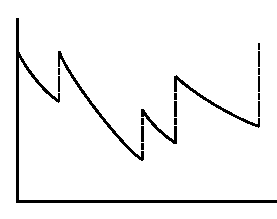
\includegraphics{vol75-figures/fig2.1.eps}
\caption{}\label{chap1:fig2.1}
\end{figure}
\end{example}

\begin{example}%%% 2.7
  \textit{A model for capacity expansion}.\pageoriginale Suppose that
  the demand for 
  some utility is monotone increasing and follows a Poisson process
  with rate $\mu$. Each `unit' of supply provides $q$ units of
  capacity. These are built one at a time at a cost of
  Rs.p. Investment takes place at a rate of Rs.$u(t)$/week and
  $u(t)\leq $ constant. When  
  $$
  \int\limits^t_0 u(s) ds = p, 
  $$
  then the project is finished, capacity is increased by $q$ and
  investments are channelled into next project.  
\end{example}

  Denote $d_t$ = demand; $c_t$ = capacity at time $t$;
  $\xi_t$ = cumulative investment in current project
$$
=\int\limits^t_\tau u(s) ds,
$$
where $\tau$ is the last time project was completed. Investment is
determined by some ``policy'' $\psi $, i.e.,  
	$$
	u(t) = \frac{d}{dt} \xi_t = \psi (c_t, d_t, \xi_t)
	$$
where $(c_t, d_t, \xi_t)$ is the current ``situation''. Define $v_t =
(c_t, d)$. Then the process $x_t = (\nu_t, \xi_t)$ evolves in the
state space $E = Z^2_+ \times [o, p]$ ($Z^2_+$ is the 2-dimensional
positive integer lattice). Then for $\nu = (c,d )$ if $g_\nu (\xi) =
\psi (c, d, \xi), \xi_t$ satisfies $\dfrac{d}{dt}\xi_t = g_{\nu_t}
(\xi_t)$.  

\medskip
\noindent{\textbf{The piecewise-deterministic process;}}

Let $K$ be a countable set and $d: K\to \mathbb{N}$ (= natural numbers)
be a given function. For each $\nu \in K, M_\nu$ is an open subset of
$\mathbb{R}^{d(\nu)}(M_\nu$ can be a $d(\nu)$-dimensional
manifold). Then the\pageoriginale state space of the $PD$ process is  
$$
E = \underset{\nu \in K }{U} M_\nu = \{ (\nu, \xi ) ; \nu \in K, \xi
\in M_\nu\}. 
$$
Let  
$$
E = \left\{\underset{\nu \in K }{\cup'} A_\nu ; A_\nu \in B(M_\nu)\right\}
$$

Then $(E,E)$ is a Borel space. Then the process is $x_t = (\nu_t,
\xi_t)$. The probability law of $(x_t)$ is specified by  
The probability law of $(x_t)$ is specified by 
\begin{enumerate}[(i)]
\item Vector fields $(X_\nu, \nu \in K)$

\item A `rate' function $\lambda: E \to \mathbb{R}_+$

\item A transition measure $Q: E \times E \to [0,1]$
\end{enumerate}
	
Assume that corresponding to each $X_\nu$ there is a unique integral
curve $\phi_\nu (t,z)$, i.e., $\phi_\nu (t,z)$ satisfies  
\begin{align*}
  \frac{d}{dt}f(\phi_\nu (t,z)) & = X_\nu f(\phi_\nu (t,z))\\
  \phi_\nu (o,z)					 & = z
\end{align*}
for every smooth function $f$, and $\phi(t,z)$ exists for all $t \geq
o$. Let $\partial M_\nu$ be the boundary of $M_\nu$. $\partial^\ast
M_\nu$ is those points in $M_\nu$ at which integral curves exit from
$M_\nu$, i.e., $\partial^\ast M_\nu = \{ z \in \partial M_\nu :
\phi_\nu (t, \xi ) = z$  for some $(t, \xi )\in \mathbb{R}
\times M_\nu \}$.   

Let 
$$
\Gamma^* = \{ \nu, z : \nu : \in K, z \in \partial ^* M_\nu\}.
$$
So $\Gamma^*$ is the set of points on the boundary at which jumps may
take place. For $x = (\nu, z) \in E$, denote  
$$
t*(x) = \inf \{ t > 0: \phi_\nu (t,z) \in \partial^\ast M_\nu\}.
$$

Write $Xh(x)$ for the function whose value at $x = (\nu, z)$ is $X_\nu
h (\nu,.)(z)$. For $\lambda$, we suppose that the function $t \to
\lambda (\gamma, \phi_\nu (t,z))$ is Lebesgue integrable on $[o,\in]$
for\pageoriginale some $ \in > 0, 0(.,x)$ is a probability measure on
$(E, E)$ for each $ x \in E U \Gamma*$.   

The motion of the process ($x_t$) starting from $x = (n, z )\in E$ is
described as follows. Define  
$$
F(t) =
\begin{cases}
   \exp \left(- \int\limits ^t_0 \lambda (n, \phi_n (s,z)) ds\right),
   & t < t^*(x)\\ 
  \qquad \qquad 0, & t \geq t^* (x). 				 
\end{cases}		
$$

This is the distributions of $T_1$, the first jump time. More
precisely, $F(t)$ is the \textit{ survivor function} 
$$
F(t) = P_x [T_1 > t].
$$


Now let $Z_1$ be an $E$-valued random variable with distribution\break $Q
(,; \phi_n) (T_1, z))$. Then define  
$$
x_t = 
\begin{cases}
(n, \phi_n (t, z)) & t < T_1\\
\quad Z_1 & t =T_1
\end{cases}
$$
and restart with ($n, z$) replaced by $Z_1$. Assume $T_k\uparrow
\infty $ a.s. Then $x_t$ defines a measurable mapping from ($\Omega,
a, P$) (countable product of unit interval probability spaces) into
space of right continuous $E$- valued functions. This defines a measure
$P_x$ on the Canonical space.  

\medskip
\noindent{\textbf{NB:}}
 The condition on $\lambda$ ensures that $T_1 > 0$ a.s and
hence that $T_{k} - T_{k-1} > 0 $ a.s.  

\begin{prop} %%%% 2.2
  $(x_t, P_x)$ is a Markov process. 
\end{prop}

\begin{proof}
  Suppose that $T_x \leq t < T_{k+1}$. The distributions of
  $T_{k+1}-T_k$ is given by  
  $$ 
  P[T_{k+1}- T_k > s]= 
  \begin{cases}
    \exp \left(- \int\limits^s_0 \lambda
    \left(\nu_{T_k},\phi_{T_k}\right)du \right), & s< t^* (x_{T_k})\\ 
    \qquad \qquad 0, & s\geq t*(x_{T_k}).
\end{cases}
$$\pageoriginale
Denote $\nu = \nu_{T_k}, \xi = \xi_{T_k} $, Then for $s > t$ and $s<
t^* (x_{T_k})$ 
\begin{align*}
  P[T_{k+l}> s | T_k, T_{k+l}> t] & = P[T_{k+l}-T_k > s-T_k | T_k,
    T_{k+l}-T_k > t- T_k]\\ 
  & = \exp \left[-\int \limits^{s-T_k}_{t-T_k}\lambda (\nu, \phi (u, \xi
    ))du\right]\\
  & = \exp \left[-\int\limits^{s-t}_o \lambda(\nu_t, \phi_{\nu_t}(u,
    \xi_t )) du\right] 
\end{align*}
where we used the semigroup property of $\phi$. Since the process
``restarts'' at $T_{k+1}$, the law of the process for $s > t$ given
part upto $t$ coincides with the law given $x_t$. Hence the Markov
Property. 
\end{proof}

Let $\Gamma \subset \Gamma^*$ be the subset for which, if $y = (\nu,
\xi )\in \Gamma^*$ 
$$
P[T_1 = T^* (x)] \to as x= (n,z) \to y.
$$
 
Then $\Gamma$ is called the ``essential'' boundary 

\begin{exercise} %Exercise 2.2
  Prove that $y \in \Gamma$ if and only if $P_x [T_1 = T^* (x) ]> 0$
  for some $ x = (\nu, z)$.  
\end{exercise}

So $P_x [x_{s-}\in \Gamma - \Gamma^*]$ for some $s > 0] = 0$, and $Q(A,
  x)$ need not be specified for $x \in \Gamma - \Gamma^*$.  

\begin{example} %Example 2.8
  Here $\nu$ has only a single value; so delete it. $\xi$ takes values
  in $M = [0.1] \times \mathbb{R}_+, \lambda = 0 $ and $X =
  \dfrac{\partial}{\partial \xi _1}$. Then $\Gamma^* = \{ (l, y); y
  \in \mathbb{R}_+\}$. Let $Q(., (l, y))= \delta (1- \dfrac{1}{2}y,
  \dfrac{1}{2}y)$.  

  Then\pageoriginale starting at $x_0 = (0,1)$ we have 
  $$
  T_n = \sum^n_{k=1}\frac{1}{k-1}\text{ so that }\lim_{ n \to \infty
  }T_n < \infty. 
 $$

  The same effect could be achieved by the combined effect of $\lambda$
  and $Q$, suitably chosen. So, we prefer to assume $T_\infty= \infty$
  a.s. rather than stating sufficient conditions on $\chi, \lambda, Q$
  to ensure this. To illustrate the difference between
  $\Gamma$ and $\Gamma^*$, suppose that $\lambda(\xi_1, 1)=
  \dfrac{1}{1-\xi _1}$ (This is equivalent to saying $T_1$ is
  uniformly distributed on [$0,1$] if the process starts at
  $(0,1)$. Then (1,1) os never hit, whatever be the starting
  point. So (1,1) $\in \Gamma - \Gamma^*$.  

\begin{figure}[H]
\centering
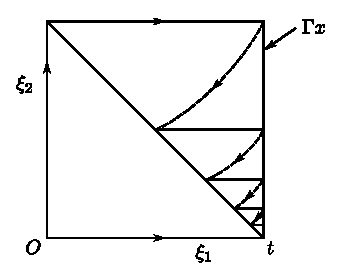
\includegraphics{vol75-figures/fig2.2.eps}
\caption{}
\end{figure}
\end{example}

\smallskip
\noindent{\textbf{The Associated Jump Process.}}		

Let ($x_t$) be an PD process. Definite the associated jump process
$(z_t)$ by  
\begin{equation*}
  z_t = x_{T_k}, t \in [T_k, T_{k+1}[\tag{2}\label{chap1:sec2:eq2}
\end{equation*}		

This\pageoriginale is an $E$-valued jump process such that $Z_{T_K} =
x_{T_K}$. Let $F_t = \sigma \{ x_s, s \leq t \}$  and $F^z_t = \sigma
\{z_s, s \leq t\}$.  

\begin{prop}% prop 2.3
  $F_t = F^z_t$ for each $t$
\end{prop}

\begin{proof}
  This follows form the fact that there is a one-to-one mapping from
  $x_{[o,t]}$ to $z_{[o,t]}. x \to z $ is given by
  (\ref{chap1:sec2:eq2}). Conversely, 
  if $z_{[o,t]}$ is given then $x{[o,t]}$ can be constructed since the
  motion in the interval $[T_k, T_{k+1}[$ is deterministic. 
\end{proof}


\medskip
\noindent{\textbf{NB:}}
\begin{enumerate}[(1)]
\item $x_t $ and $z_t$ are not in one-to-one correspondence at each
  fixed time $t$.  

\item $(z_t)$ is not a Markov process. 
\end{enumerate}
Since $F_t = F^z_t$, we can apply jump process theory. Define 
\begin{align*}
  p(t,A) &=  \sum\limits_{T_i \leq t}  I_{(x_{T_i}- \in  A)}\\
  p^*_t &= \sum\limits_{T_i \leq t}  I_{(x_{T_i}- \in  \Gamma)}\\
  \tilde{p}(t, A) &= \int\limits_0^t Q(A, x_s ) \lambda (x_s) ds +
  \int\limits_0^t Q(A, x_s\_)dp^*_s \tag{3}\label{chap1:sec2:eq3} 
\end{align*}

\begin{prop}\label{chap1:prop2.4}% prop 2.4
  Suppose  $E(p (t, E))< \infty $. Then for each
  \begin{equation}
    A \in  E, q (t, A) = p (t,A) - \tilde{p}(t,A) \tag{4}\label{chap1:sec2:eq4}
  \end{equation}
    is an  $F_t$-martingale.
\end{prop}

\begin{proof}
  From previous results, the compensator of $p (t \Lambda T_1, A)$ is 
  $$
  \tilde{p}(t \Lambda T_1, A) = -\int\limits_{] o, t \Lambda T_1 ]} Q
  (A, x_{s-}) \frac{dF_s}{F_{s-}}. 
  $$
  
  But\pageoriginale  
  $$
  F_t = 
  \begin{cases} 
    \exp \left(- \int\limits_0^t \lambda(x_s)ds \right) & \quad t < t^*_1(x)\\
    0 & \quad t \geq t^*_1 (x).
  \end{cases}
  $$

  Thus -$\dfrac{dF_t}{F_t } = \lambda (x_t) dt$ for $t < t^*_1 (x) $ and 
  $$
  \frac{\triangle F_{t^*_t}}{F_{t^*_1}-} = 1.
  $$
\end{proof}

This verifies the result for $t \leq T_1$. As before, we show by
considering intervals $[T_{k-1}, T_k ]$ that the compensator of $p (t
  \Lambda Tn, A )$  is $\tilde{p}(t \Lambda T_n, A)$ given by
  (\ref{chap1:sec2:eq3}). Since $p(t,A)$ and $\tilde{p} (t, A)$ are monotonic
  increasing functions and $T_n \uparrow \infty$ a.s. $E (p(t,E)) <
  \infty$, taking the limits, we have  
  $$
  q(t,A) = p(t,A)- \tilde{p} (t,A)
  $$
  is a martingale.

\begin{exercise} % exe 2.3
  Show that $p^*_t $ is an $F_t-$ predictable process. 
\end{exercise}

Then (\ref{chap1:sec2:eq4}) is the Doob-Meyer decomposition of the
submartingale $p$.  

The next step is to use stochastic integrals to calculate the extended
generator of $x_t$. Choose the following integrands. For Measurable
$f: \bar{E} \to \mathbb{R}$, define  
$$
Bf(x,s,\omega) = f (x) - f(x_{s-} (\omega))
$$

Then Bf $\in  L_1 (p)$ if 
$$
E \sum_{T_i \leq t}| f(x_{T_i})- f(x_{T_i-})| < \infty 
$$
for\pageoriginale each $t \geq 0$. This certainly holds if $f$ is
bounded and $E ~p ~(t, E ) < \infty$.  
\begin{multline*}
  \int\limits_o^t \int\limits_E Bf(y, s,w) \tilde {p} (ds,dy) =
  \int\limits_{[ 0, t ]} \int\limits_{E} (f(y) - f(x_{s-}))
  Q(dy;x_{s-}) \lambda (x_s)ds\\ 
  + \int\limits_{[ 0, t ]} \int\limits_{E}(f(y) - f(x_{s-}))
  Q(dy;x_{s-})ds_{s}. \tag{5}\label{chap1:sec2:eq5} 
\end{multline*}

Suppose that $f$ satisfies the boundary condition 
\begin{equation*}
  f (x) = \int\limits_{E} f (y) Q (dy; x), x ~\in  ~
  \Gamma. \tag{6}\label{chap1:sec2:eq6} 
\end{equation*}

Then the second integral in (\ref{chap1:sec2:eq5}) is zero. The
following result characterizes the extended generator $A$ of $(x_t)$.  

\begin{theorem} % 2.1
  The domain  $D(A)$ of the extended generator  $A$ of $(x_t)$ consists
  of those functions $f$ satisfying  
  \begin{enumerate}[(i)]
  \item For each  $(n,z)~\in ~ E$   the function 
    $t \to f (n, \phi_n (n, z))$ is absolutely continuous for 
    $t \in  [0, t^* (n, z)[$.  

    \item The boundary condition (\ref{chap1:sec2:eq6}) is satisfied.

    \item Bf $\in ~ L^{\loc}_1 (p)$.
  \end{enumerate}
  Then for $f~ \in ~ D (A)$
  \begin{equation*}
    Af(x) = Xf(x) + \lambda (x) \int\limits_{E} [f(y) - f(x)] Q (dy;
    x).\tag{7}\label{chap1:sec2:eq7} 
  \end{equation*}
\end{theorem}

\begin{proof}
  Suppose that $f$ satisfies (i)-(iii). Then $\int$ Bf $dq$ is a
  local martingale, and  
{\fontsize{10pt}{12pt}\selectfont
  \begin{gather*}
    \int\limits_0^t Bf dq =\sum_{T_i \leq t } f (x_{T_i}) - f(x_{{T^-}_{i^-}})
    -\int\limits^t_0 \int\limits_{E} [f (y) - f (x_s )] Q (dy; x_s)
    \lambda (x_s ) ds. 
  \end{gather*}}\relax

  Now,\pageoriginale 
  \begin{multline*}
    \sum_{T_i \leq t } f(x_{T_i}) - f(x_{T_{\bar{i}}}) = \left[ \sum_{T_i
        \leq t } (f (x_{T_i }) - f(X_{T_{i-1}})) + f (x_t) - f
      (x_{T_n})\right]\\ 
    -\left[\sum_{T_i \leq t } (f(x_{{T^-}_{\bar{i}}}) - f(x_{T_{i-1}})) + f
      (x_t) - f (x_{T_n})\right] 
  \end{multline*}
  where $T_n $ is the last jump time before $t$. The first bracket is
  $(f(x_t)- f(x_o))$. Note that  
  $$
  f(x_{T_{\bar{i}}}) - f(x_{T_{i - 1}}) = \int\limits^{T_i}_{T_{i -
      1}} X_{\nu_{T_{i-1}}} f (\nu_{T_{i - 1}}' \phi_{\nu_{T_{i - 1}}} (\xi
  T_{i - 1},s) ds~ \text{a.s}).   
  $$
\end{proof}

So the second bracket is equal to $\int\limits^t_0 x f (x_s )ds $ and 
\begin{multline*}
\int Bf dq = f(x_t ) - f (x_0 ) -\\ 
\int \limits^t_o \int\limits_{E}
(f(y)- f(x_s)) Q (dy, x_s) \lambda (x_s) ds - \int\limits^t_o X f (x_s
)ds. 
\end{multline*}

So $Af$ is given by (\ref{chap1:sec2:eq7}) and $C^f_t = \int\limits^t_0$ Bf
$dq$. Conversely, suppose $f~ \in ~ D(A)$. Then there exists a
function $h$ such that $s \to h (x_s)$ is Lebesgue integrable and $M_t
= f(x_t ) - f(x_0 ) - \int\limits^t_0 h(x_s)ds$ is a local
martingale. By the martingale representation theorem, $M_t = M^g_t$
for some $g~ \in  ~L^{1oc}_1 (p)$. Now the jumps of $M_t$ and
$M^g_t$ must agree, these only occur when $t = T_i $ for some $i$ and
are then given by  
\begin{align*}
  \triangle M_t & = M_t - M_{t-} = f(x_{T_i}) -f(x_{T_{\bar{i}}}).\\
  \triangle M^g_t & = M^g_t - M^g_{t-}\\
  & = g(x_t, t,w ) - \int\limits_{E} g (y,t,w) Q (dy, x_{t-})
  I_{(x_{t- } \in  \Gamma)} 
\end{align*}
at $t = T_i $. It follows that 
$$ 
g (x,t,w) I_{(x_t \notin / \Gamma)} = (f(x) - f(x_{t-})) I_({x_{t-
    \notin \Gamma)}} 
$$\pageoriginale
except possibly on a set $G \in E * p$ such that 
$$
E_y \int \limits_{\mathbb{R}_+ \times E} I_G p(dt, dx) = 0 \text{ for
  all } y~ \in ~ E. 
$$

Now suppose $X_{T_i} = z \in \Gamma$; then
$$
f(x) - f(z) = g(x,t,\omega) - \int \limits_E g (y, t, \omega) Q(dy ; z)
$$
for all $x$ except a set $A~ \in~ E$ such that $Q (A,z) = 0$. Since
only the first terms on the left and right involve $x$ it must be the
case that  
$$
\displaylines{\hfill 
  f(x) = g(x,t,\omega) + \tilde{f} (t,\omega)\hfill \cr
  \text{and}\hfill  
  f(z) = \int \limits_E g(y,t,\omega) Q(dy ; z) + \tilde{f}(t, w)\hfill }
$$
for some predictable process $\tilde{f}$. Since $g = f - \tilde{f}$, 
$$
f(z) = \int \limits_E f (y) Q(dy ; z)
$$
for $z~ \in~ \Gamma$, i.e., $f$ satisfies condition (ii). Hence 
$$
g(x, t, \omega) = f(x) - f(x_{t-}).
$$

Hence we get 
$$
\| (Bf - g ) I_{(t < \sigma_n)} \| L_1 (p) = 0.
$$

So condition (iii) is satisfied. Fix $\omega$ and consider
$(M_{t})_{o \le t < t_1(\omega)}$ starting at $(\nu_o, \xi_o)^.$, then  
\begin{align*}
  M_t & = f(\nu_o, \phi_{\nu_o} (t, \xi_o)) - f(\nu_o, \xi_o) - \int
  \limits^t_o h (x_s) ds \\ 
  M^g_t & = \int \limits^t_o \int \limits_E (f(y) - f(x_s)) Q (dy ;
  x_s) \lambda(x_s) ds.  
\end{align*}

Hence $f(\nu_o, \phi_{\nu_o} (t, \xi_o))$ is absolutely continuous for
$t < T_1(\omega)$. 
Since\pageoriginale $(\nu_o,\xi_o)$ is arbitrary and $T_1(w) > 0$
a.s. this shows that (i) is satisfied. 


\medskip
\noindent{\textbf{A ``Feynman-Kac'' formula.}}

This is used to calculate expected values of functionals such as
$$
E_x\left[\int\limits_o^t ~ e^{-\alpha s} ~ c(s,x_s)ds + e^{-\alpha t}
  ~ \phi(x_t)\right]. 
$$

There is no extra generality in allowing a $P.D$. Process to be
time-varying, because time can always be included as one component of
$\xi_t$. However, it is sometimes convenient to consider the joint
process $(t, x_t)$ with generator $\tilde{A} =
\dfrac{\partial}{\partial t} + A$. Then for $f ~\in  ~D
(\tilde{A})$ 
$$
f(t,x_t) - f(o,x_o) = \int\limits^t_o ~ \left(\frac{\partial}{\partial s} +
A\right) f(s,x_s)ds + \int\limits_o^t ~ Bf ~ dq. 
$$

If $\left(\dfrac{\partial}{\partial s}+A\right) ~ f(s,x_s) = o$ and $Bf ~
\in  ~ L_1(p)$, then $f(t,x_t)$ is a martingale, so it has
constant expectation 
$$
E_{x_o}~ f(t,x_t) = f(o,x_o).
$$

Then
$$
\displaylines{\hfill 
  f(o,x_o) = E_{x_o} ~ \phi(x_t)\hfill \cr
  \text{where}\hfill 
  f(t,x) = \phi(x) \quad (\phi ~ \text{ prescribed}).\hfill}
$$

\begin{prop}\label{chap1:prop2.5}% PROP 2.5
  Let $t > o$ be fixed and $\alpha : [o, t] \times E\rightarrow
  \mathbb{R}_+, c:[o,t] \times E \rightarrow \mathbb{R}$ and $\phi: E
  \rightarrow \mathbb{R} $ be measurable functions. Suppose $f : [o,
    t] \times E \rightarrow \mathbb{R} $ satisfies: 

\begin{equation*}
  \left.
    \begin{aligned}
      {\rm (i)} \qquad  & f(s,. \in D (\tilde{A})) \\
      {\rm (ii)} \qquad  & f(t, x) = \phi (x), \; x \in E \\
      {\rm (iii)} \qquad  & Bf \in L_l (p) 
    \end{aligned} \qquad 
  \right\} \hspace{4cm}  \tag{8}\label{chap1:sec2:eq8}
\end{equation*}

  \begin{gather*}
    \frac{\partial f(s,x)}{\partial s} + Af(s,x) -\alpha
    (s,x)f(s,x)+c(s,x) = 0 \tag{9}\label{chap1:sec2:eq9}\\ 
    (s,x) ~ \in  ~ [o,t[ ~ \times E.
  \end{gather*} \pageoriginale
Then
\begin{multline*}
f(o,x) = E_{o,x}\left[\int\limits_0^t \exp \left(-\int\limits_o^s
  \alpha (u,x_u)du \right) c(s,x_s)ds\right.\\ 
  \left. + \exp \left(-\int\limits_o^t
  \alpha(u,x_u)du\right)\phi(x_t)\right]\tag{10}\label{chap1:sec2:eq10} 
\end{multline*}
\end{prop}

\begin{proof}
Suppose $f$ satisfies (\ref{chap1:sec2:eq8}). Define
$$
e_s = \exp \left(-\int^s_o \alpha(u,x_u)du\right).
$$
Then
\begin{align*}
  d(e_sf(s,x_s)) & =  e_sdf(s,x_s) + f(s,x_s)de_s\\
  & = e_s\left(\frac{\partial f}{\partial s} + Af\right)ds + e_s ~ Bf ~ dq
  -\alpha (s, x_s)e_sf~ds\\ 
  & = -e_s ~ c(s,x_s)ds + e_s ~ Bf ~ dq ~\quad \text{(by
  (\ref{chap1:sec2:eq9}))}. 
\end{align*}
Now by (iii), $e_s ~ Bf ~ \in  ~ L_1(p)$ since $e_s \leq
1$. Thus the last term is a martingale and 
$$
E_x[e_tf(t,x_t)-f(o,x)] = - E_x\left[\int\limits_o^t e_sc(s,x_s)ds\right].
$$
This with (ii) gives (\ref{chap1:sec2:eq10}).
\end{proof}

\begin{example}%Exmp 2.9
  \textit{The Renewal Equation:}

  Let $(N_t)$ be a renewal process with inter arrival density
  $f(.)$. Let $m(t) = EN_t$. Since the process ``restarts'' at renewal
  times, 
  \begin{equation*}
    E[N_t | T_1 = s] = 
    \begin{cases}
      0, & s > t\\
      m(t-s)+1, & s < t.
    \end{cases}
  \end{equation*}
So
$$
m(t) = \int\limits^\infty_o E[N_t | T_1 = s] ~ f(s)ds
$$\pageoriginale
which gives the renewal equation
\begin{equation*}
m(t) = \int\limits^t_o (1+m(t-s)) f(s) ~ ds.\tag{11}\label{chap1:sec2:eq11}
\end{equation*}
This can be solved by Laplace transforms. Defining
$$
\hat{f}(p) = \int\limits^\infty_o e^{-pt} f(t) dt
$$
etc., we get 
$$
\hat{m}(p) = \hat{m}(p) ~ \hat{f}(p) + \frac{1}{p} ~ \hat{f}(p). 
$$
So   
$$
\hat{m}(p) = \frac{\frac{1}{p}\hat{f}(p)}{1 - \hat{f}(p)}.
$$
In particular, for the Poisson process $f(t) = \lambda e^{-\lambda
  t}$, 
$$
\hat{f} = \frac{\lambda}{\lambda + p}
$$
will give
$$
\hat{m} (p) = \frac{\lambda}{p^2}
$$
to get
$$
m(t) = \lambda t. 
$$
\end{example}

\begin{exercise}\label{chap1:exer2.4}% exercise 2.4
  Compute $M_{\tauup}(t) = E_\tauup N_t$, where the component in
  service at time 0 has age $\tauup$ (and is replaced by a new
  component when it fails). 
\end{exercise}

$(N_t)$ is a $PD$ process if we take $x_t = (\nu_t,\xi_t)$ where
$\nu_t = N_t$ and $\xi_t$ is the time since last renewal. Then 
$$
X_\nu = \frac{\partial}{\partial \xi},\quad \lambda(\xi) =
\frac{f(\xi)}{\int\limits^\infty_\xi f(u)du} 
$$
and\pageoriginale $Q(.; \nu, \xi) = \delta_{(\nu + 1,0)}$, so that 
$$
Af(\nu,\xi) = \frac{\partial}{\partial \xi} f(\nu,\xi) +
\lambda(\xi)[f(\nu + 1,0) - f(\nu,0)]. 
$$
Use proposition \ref{chap1:prop2.5} with $\alpha = c = 0$ and $\phi(x)
= \nu$ to get  
$$
f(0,\nu,\xi) = E_{(\nu,\xi)} \nu_t.
$$
Clearly 
$$
f(s,\nu + 1, \xi) = f(s,\nu,\xi ) + 1.
$$
Define
$$
f(s,0,\xi) = h(s,\xi).
$$
Then the equation for $f$ (or $h$) becomes
\begin{gather*}
  \frac{\partial}{\partial s} h(s,\xi ) +\frac{\partial}{\partial \xi}
  ~ h(s,\xi) + \lambda(\xi)[1+h(s,0)-h(s,\xi )] = 0
  \tag{12}\label{chap1:sec2:eq12} \\  
  h(t,\xi ) = 0.  
\end{gather*}
Define
$$
z(u)= h(u,u).
$$
Then
\begin{align*}
\frac{d}{du} z(u) & = -\lambda(u)[1+h(u,0) - z(u)]\\
z(t) & = 0.
\end{align*}
Thus $z(u)$ satisfies
\begin{equation*}
\dot{z}(u) = \lambda(u) ~ z(u) -\lambda(u) [1 +
  h(u,0)]\tag{13}\label{chap1:sec2:eq13} 
\end{equation*}
where
$$
\lambda(u) = - \frac{\dot{F}}{F} = \frac{f}{F}, F(u) =
\int\limits^\infty_u f(s) ~ ds. 
$$
Equation (\ref{chap1:sec2:eq13}) is a linear $ODE$ satisfied by
$z(u)$. The transition function corresponding to $\lambda(u)$ is   
$$
\phi(u,v) = \frac{F(u)}{F(v)}
$$

Hence\pageoriginale (\ref{chap1:sec2:eq13}) has the following solution
at time 0: 
\begin{equation*}
  z(o) = h(o,o) = \int\limits_o^t
  f(u)[1+h(u,o)]du\tag{14}\label{chap1:sec2:eq14} 
\end{equation*}
Define
$$
m(s) = h(t - s,o).
$$

Then (\ref{chap1:sec2:eq14}) coincides with the renewal equation
(\ref{chap1:sec2:eq11}). Having determined $h(u,o)\, o \le u \le
t,h(s, \xi)$ for $s \neq \xi \neq o$ can be calculated from
(\ref{chap1:sec2:eq12}). The result will be equivalent to that of
Exercise \ref{chap1:exer2.4}.  


